\documentclass{article}
\usepackage[utf8]{inputenc}
\usepackage{float}
\usepackage[margin=0.8in]{geometry}
\usepackage{graphicx}
\graphicspath{ {img/} } 


\title{WebApp Final Report}
\author{Chase Hellemans. Beatrix de Wilde, Gagan Kaur, Henry Cuttell}
\date{June 2015}

\begin{document}

\maketitle

\section{Introduction}
\subsection{Description of our Application}
The problem we are addressing is when a group of friends want to watch a film together, it can often take a long time for them to decide which film everybody wants to watch. As a group, we have all been in this situation many times and so we really wanted to create an app to address this problem. Our web application, NextFlick, aims to greatly reduce the time and number of debates (sometimes arguments) it takes for a group of friends to decide on which film to watch. 

The concept is simple; we show films to each user to which they respond with ‘yes’ or ‘no’. When a consensus has been reached, the application will immediately alert all of the users to the chosen film. This means the decision process is shortened massively (everyone’s decision for each film is made individually so the decision can be made swiftly), it also stops people from being pressured into watching films they don’t want to watch.

Our aim was to create an app with a fluid user interface, allowing the user to get started with as few clicks through to film selection as possible. This is because any small amount of inconvenience in our application will draw users away as the application should take no longer than it normally takes in person. We also wanted an intuitive lobby system, with users easily being able to tell if they have successfully connected to the correct session.

The process a group of people will follow when using the application is as follows:

One user will act as the leader and create a session, this will take them to a lobby page when their room ID is displayed, along with film filtering options such as film genres and run-time filters (leader only). The other users in the group will then join this session using the unique ID of the session (the group leader tells them this ID) and then select their film genre preferences, clicking ‘ready’ when they are finished.

The leader can then click ‘go’ to start the session, sending all users to the film selection page where they begin selecting ‘yes’ and ‘no’ for each film they are presented with. When all users have said ‘yes’ for a given film, they will be taken to a session complete page when the chosen film is displayed. They can then either quit the app or choose to create or join another session.

\subsection{Requirements}
\begin{itemize}
\item Cross-platform compatibility between mobile and PC - as most users will want to use their phone, but some users will use their computers (usually the streaming computer)
\item Fast and convenient access, joining or creating should be no more than 2-3 clicks
\item Users should just be use the application quickly regardless whether it is the user’s first time or not
\item Users should be able to vote on a film at their own pace without being restricted by other users
\item Users should be able to make a choice on a film as fast as possible, with the possibility of swiping for mobile and left and right keys for PC
\item Transitions from one page to the next should be smooth and not confuse the user
\end{itemize}
\section{Project Management}
\subsection{Group Structure}
We used Trello in order to coordinate who was working on which features and to keep track of the level of completion. It was also a good tool to store a list of additional features that could be added if time allowed. In order to collaborate on the presentation and reports google docs was used. 

For the majority of this project our whole group has been working in labs. This allows us to discuss progress on the web app easily. Working in labs also means we can pair program meaning not just one group member exclusively understands one aspect of the application. 

We decided on an idea during a brainstorming session with the whole group. After this and discussing initial plans for the web application we split the work on what everyone wanted to do. Beatrix, the project manager, focused on the interaction between the server and the database. She created the user table and popular films table in the database and implemented user sign-up and login. Gagan concentrated on user interaction with the web application. She mainly worked on the user interface and client side processing. Chase worked on connection between the client and the server. He focused on the room creation, processing and tear down on the server side. While also working on how this is displayed to the user and showing whether or not a user has made their filter preferences. Henry worked on the connection between the server and the two APIs (TMDb and OMDb). He also implemented how films are stored and processed on the server end and the filtering of the films for the different genre and run time preferences.
\subsection{Implementation Languages}

\subsubsection{JavaScript}
JavaScript is an extremely powerful language and we are using it as our back-end with Node.js and Socket.io. We also use jQuery to easily manipulate HTML elements - which is used to control the elements of our Single-Page Application. Since both the control of the client and the server are both in the same language, it will be easier to read. 

\subsubsection{Node.js}
Node.js has a plethora of useful libraries (more in section~\ref{subsec:nodelibraries}) concerning web applications that we used in our own Web App. Furthermore, putting our application on the server will be extremely easy as we are using Node.js.

\subsubsection{Socket.io}
Socket.io makes client and server communication simple to use as well as the fact it is easily integrated with JavaScript. Our application is Single-Page Application and Socket.io was built with long polling in mind, making it the best choice. Socket.io abstracts many transport layers and simplifies the use of WebSockets and since our group had no experience in using sockets prior this project, it was easy for us to learn and use it in exactly the way that we wanted. 
\subsubsection{postgreSQL}
We chose to use the given postgreSQL database. Firstly we chose to use a SQL based database over noSQL as it has more community support. Also most of the groups knowledge lies with SQL and it has more integrity checks. Secondly we chose a postgreSQL database to ensure data reliability and stability. This is essential for us as we store user email addresses which is considered personal data as a person can be identified from their email address. Therefore due to the data protection act this data needs to be stored securely against unauthorised or unlawful processing. 
\subsection{Design Processes}
Our design process consisted of the following steps:
\begin{enumerate}
\item We first had to decide on an idea for the web application, we did this in an initial group meeting.
\item In order to start working, we implemented a skeleton webpage where we could display the core functionality of our app as it was implemented.
\item We then decided on a feature to add and discuss as a group whether this is a good idea and fit for the application.
\item We allocate a team member to work on the feature and thoroughly test it before pushing to our master branch on git (we used a separate branch to work on large features).
\item Back to step 3 (decide on another feature to add).
\item We regularly showed our app to other people to get feedback and ideas for future features.
\item Once we had implemented all of the features we wanted our app to have, we showed our app to more users for more feedback. If any new features were suggested we would go to step 3.
\end{enumerate}

\subsection{Version Control}
We decided to use GitHub as a version control and backup system. This made it easy for us to collaborate and merge our work and meant our work was backed up at every point. It was also helpful to be able to go back to a previous state of our project.

\section{Program Description}
\subsection{Implementation}
\subsubsection{Database}
In our database we store a table for users and a table for the most popular films. 

The table structure~\ref{tab:usertable} shows how we store the user’s information in the database. The username and password are just for logging in. The array of genres is used to set the user’s default genres in order to perform quick filtering of films. The email is used if the user wants to change passwords.

\begin{table}[h]
\centering
\caption{User table}
\label{tab:usertable}
\begin{tabular}{|l|l|l|l|l|}
\hline
username & password & genres                        & e-mail  & films\_chosen        \\ \hline
user2    & pass2    & \{Action, Adventure, Comedy\} & user2@gmail.com & {76341,13, 205596 } \\ \hline
\end{tabular}
\end{table}

The popular films database stores the films that have been suggested most for a room to watch. Once more than a certain number of films are stored films with a small count or the last updated films are deleted. The popular films are then displayed in the lobby page. The table structure below has a unique constraint on the \texttt{film\_id} so a film does not have two entries. 

\begin{table}[h]
\centering
\caption{Popular Films Table}
\label{filmtable}
\begin{tabular}{|l|l|l|l|}
\hline
film\_id & count & poster\_url & last\_time\_updated     \\ \hline
245891 & 3 & http://image.tmdb.org/t/p/\dots & 2015-06-04 22:01:27.607 \\ \hline
\end{tabular}
\end{table}

\subsubsection{Server and Client Interactions}
Connection between client and server occur using Socket.io functions and JavaScript callback functions using JavaScript scripts (\texttt{public/script.js} and \texttt{server.js} respectively). Almost all of the application’s computations are done on the server-side, however we are cautious about the amount of data that needs to be sent to the client. 

The server keeps track of the users per channel including a lot of meta-data about each channel (e.g. whether the room is already in session, the preferences collected by the users, etc.) in 2D arrays and makes calls to various APIs to collect information about films to display to the users. The films are stored server-side as a global list and clients maintain an index into that list. Client to server interactions include requesting the next film information, logging in (or being assigned a guest ID), signing up, creating rooms and sending preferences. The server will then callback to the client to update the UI after the request has been handled. 

Server to client interactions include mainly updating aspects of the UI as well as moving on to the different pages once the films have been fully computed, or a film has been selected. Since this application is a single-page application, some movements from page to page may need to be monitored by the server - an example of this is with the Film Page; if the films were not ready for the client to display to the users, there would be a waiting overlay before the transition takes place, signalled by the server. 

The heaviest part of user interactivity is during the Film Page, each time a user makes a choice ('yes' or 'no') about a film, the client sends this choice as well as the index into the global film list. The server handles this request, dealing with it appropriately by filtering the films (more detail in section~\ref{subsubsec:api}) or getting more films in advance before the user reaches the end of the global list behind the scenes. This allows for lazy loading and for the user to have to interact as little as possible to intuitively complete their actions.
\subsubsection{API Calls and Storing of Films}
\label{subsubsec:api}
Getting the film information is a critical part of our web application so we researched different APIs to use in order to access and display this information. The main data we needed was the film title and poster image URL to display to users. We gain this information for batches of films at a time (ordered by popularity) from the TMDb (The Movie Database) API. However this API doesn’t provide us with extra film information we need such as a short synopsis, the run-time, and IMDb rating for each film. This means for each film we need to send an extra API request to the OMDb (The Open Movie Database) API which provides this information. The reason we don’t solely use the OMDb API is because it only supports querying of information for specific films, and as we needed batches of popular films this wasn't suitable. 

The hybrid solution of using both APIs gives us the ability to query for a general selection of films but also enabling us to access more in depth information for each film which we need to display to the user and filter on.

Our initial approach to storing the film information was to send TMDb API requests on demand when the user ran out of films. This meant we had to store all of this film information per user session, as well as sending the API requests repeatedly for every new session. Therefore we were storing a great deal more information than was necessary, as it was not possible to store this information once because it the results returned depended on the genres passed to each request. With this method we did however cache the OMDb requests using node-cache, as we could check if the film ID was already in the cache (if so, the request would not be resent and it would be accessed immediately from the cache).

Unfortunately we ran into problems with this implementation because it restricted our ability to filter the results effectively (we had to store an valid property with the film information to see if it had been filtered out). Also, sending the API requests for each session repeatedly is less scalable and slows down the loading of the session’s film list.

Therefore the solution to this which we implemented is to store the films just once in an array which can be accessed by all the sessions, greatly reducing the amount of memory required and speeding up the filtering process. To implement this we query the TMDb API without specifying any genre parameters, hence obtaining a list of all the films (in popularity order) of all genres. The genres are then filtered locally which means no more API requests need to be sent once the film list has been stored, greatly improving the filtering speed and scalability of the application.

Filtering the films locally also means more specific filtering can be applied easily such as film runtime constraints (e.g. only show films less than 2 hours long). This also means the genres being shown to the user can be easily changed on the fly. This implementation does however require a longer start-up phase where the TMDb API is queried for a larger batch of films. We can’t get around this because the API states you shall not: “Cache any TMDb metadata or photos other than for reasonable periods in order to provide your service”. This prohibits us from storing the film data in our database and so we have to access it via the API each time the server is started.
\subsection{Expected User Interactions}
\subsubsection{User Journey}
\begin{figure}[H]
\centering
\caption{Expected User Interaction Flow}
\label{sec:sysarchitecture}
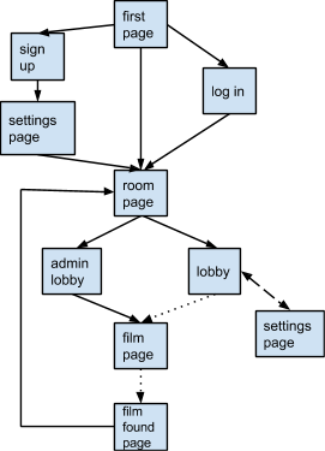
\includegraphics[scale=0.6]{userinteraction}
\end{figure}
\subsubsection{First Page}
\begin{figure}[H]
\centering
\caption{First Page}
\label{sec:sysarchitecture}
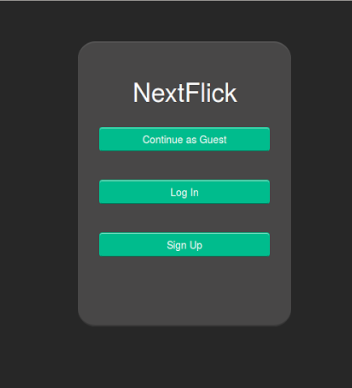
\includegraphics[scale=0.5]{firstpage}
\end{figure}
On the first page, users can choose between continuing as guest, logging in or signing up.

Continuing as guest takes you to straight to the room page.
\subsubsection{Login Page}
\begin{figure}[H]
\centering
\caption{Login Page}
\label{sec:sysarchitecture}
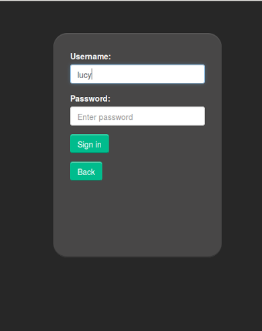
\includegraphics[scale=0.60]{loginpage}
\end{figure}
Logging in takes you to the login page where you put in your details and then goes to the room page. 
\subsubsection{Sign up and Settings Page}
\begin{figure}[H]
\centering
\caption{Sign up Page}
\label{sec:sysarchitecture}
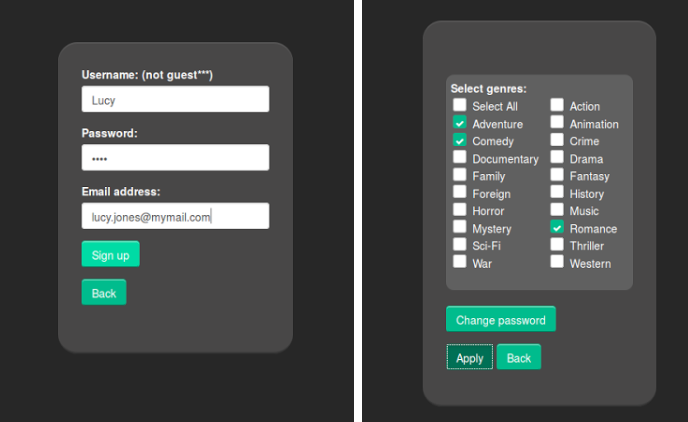
\includegraphics[scale=0.5]{signuppage}
\end{figure}
Signing up means you have to make an account and set your preferences for your genres. You are then taken to the room page.
\subsubsection{Room Page}
\begin{figure}[H]
\centering
\caption{Room Page}
\label{sec:sysarchitecture}
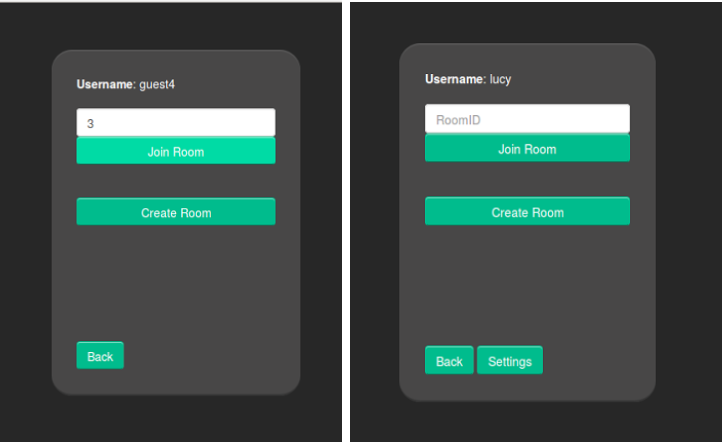
\includegraphics[scale=0.5]{roompage}
\end{figure}
On the room page you have the choice of creating a room or joining one. If you are a user you can go and edit the your settings. Creating a room makes you the admin of it and joining an existing room makes you a member of the group. You are taken to the lobby page. 
\subsubsection{Lobby Page}
\begin{figure}[H]
\centering
\caption{Lobby Page}
\label{sec:sysarchitecture}
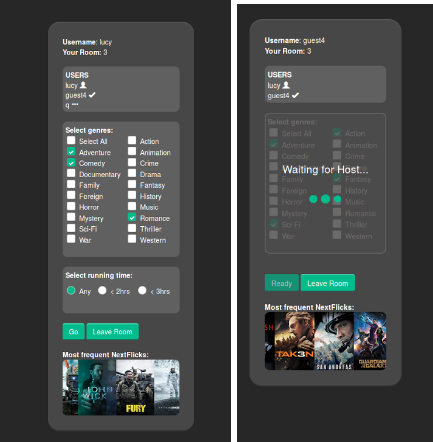
\includegraphics[scale=0.5]{lobbypage}
\end{figure}
All users can then pick which genres they are interested in, if you are a registered user your saved preferences come up. If you are not the admin you can click the ready button and have to wait for the admin to start the selection process. The admin can click go at any point and can see when the rest of the room is ready. Clicking go starts the selection process for the entire room. While the users are waiting for the rest of the room to be ready they can watch the scrolling pictures at the bottom of the screen which shows the most popular films that have been selected.
\subsubsection{Film Page}
\begin{figure}[H]
\centering
\caption{Lobby Page}
\label{sec:sysarchitecture}
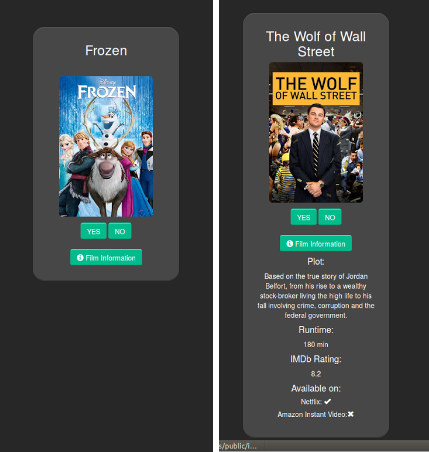
\includegraphics[scale=0.5]{filmpage}
\end{figure}
The selection process happens on the film page. Films generated using the filters the users have imposed come up one at a time and the users can say ‘yes’ or ‘no’. As soon as there is a film that all users have said yes to that film is selected and all members of the room are taken to the film found page. There is a film information box which can be expanded to show the plot, runtime, IMDb rating and whether it is available to stream on Netflix or Amazon Instant Video. 
\subsubsection{Film Found Page}
\begin{figure}[H]
\centering
\caption{Lobby Page}
\label{sec:sysarchitecture}
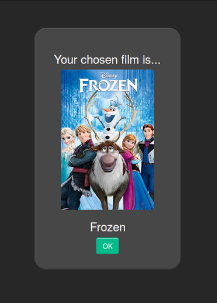
\includegraphics[scale=0.5]{filmfoundpage}
\end{figure}
The film found page displays the chosen film and when the users select OK they are taken back to the room page.
\subsection{Design Patterns}
We used the Command Queue design pattern for the OMDb API requests because it only permitted us to make 20 simultaneous requests at a time. Therefore we used the queue from the module ‘async’ where we push the API requests to, with it executing them for us. It also enabled us to set a maximum concurrency limit of 20 to prevent requests from failing because of the API limit. We had to add a callback to the function that sent off the OMDb requests so the queue knows when each request has finished.
\subsection{System Architecture}
\begin{figure}[H]
\centering
\caption{System Architecture}
\label{sec:sysarchitecture}
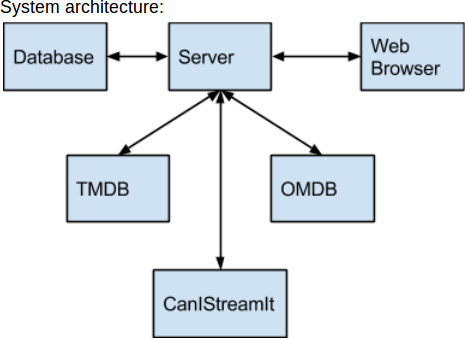
\includegraphics[scale=0.5]{sysarchitecture}
\end{figure}
%\subsection{Screenshots}
\section{Acknowledgements}
\subsection{Libraries}
\label{subsec:nodelibraries}
The “socket.io” library allowes our server and client to communicate in real time. Therefore it is used in both the server and client code. The license that the socket.io library is under is the MIT license (discussed below) with “Copyright (c) 2014-2015 Automattic \textless dev@cloudup.com\textgreater ”.

The “express” library gives us a web framework for our server. This library uses the MIT license with “Copyright (c) 2009-2014 TJ Holowaychuk \textless tj@vision-media.ca\textgreater \  Copyright (c) 2013-2014 Roman Shtylman \textless shtylman+expressjs@gmail.com\textgreater \ Copyright (c) 2014-2015 Douglas Christopher Wilson \\ \textless doug@somethingdoug.com\textgreater ”.

The “request” library is used to make API GET requests from the server to the TMDb and OMDb APIs. The film information is returned to us in JSON format, which we process and use to display and filter the films for our application. The library uses the Apache 2.0 license.

The “pg” library is imported and then used as a PostgreSQL client for node.js. This library makes it easier to connect to the postgreSQL database from the server as most of the code in the server is JavaScript. The license connected to this library is the MIT license (discussed below) with “Copyright (c) 2010-2015 Brian Carlson (brian.m.carlson@gmail.com)”. 
The library “bcrypt-nodejs” is imported in order to encrypt the user passwords. The salt generation function and hash function means we can securely store the passwords. With no way of attaining the original password from the hash stored in the database. This library also uses the MIT license  (discussed below) but with “Copyright (c) 2010 Nicholas Campbell”. 

The “async” library is used to provide a queue for the OMDb API requests on the server side and to set a concurrency limit of 20 simultaneous requests (maximum the API allows). This is to stop us exceeding this limit and sending additional requests which will fail. The library uses the MIT license (discussed below) with “Copyright (c) 2010-2014 Caolan McMahon”.

The “nodemailer” library is used to send emails on the server side to the user in order for them to change their password. An email with a random number is sent to the stored user email address then in order for the user to change their password this number is entered in with their old and new password. The nodemailer library is also under the MIT license (discussed below) with “Copyright (c) 2011-2015 Andris Reinman”. 



The Hammer.js library has been included in the client side so we can use swipe (swipe right = yes, swipe left = no) with our web app. We considered using the jquery mobile library but it included code that would override some of our style code. This library is under the MIT license (discussed below).

We included the bootstrap stylesheet to make our website responsive and easy to style for mobile. It included lots of nice style elements which we could then adapt to fit our application.   Bootstrap is under the MIT license (discussed below).

The file awesome-bootstrap-checkbox.css and the font-awesome library were included for the custom checkboxes. We used this as we felt the default checkboxes didn’t fit with our application and this library allowed us to easily change them. This code was licenced under the MIT licence.

The MIT license allows us to use any library under it without restriction as long as we include the copyright and permission notice connected with the software. As we require these libraries and the libraries contain their respective licenses with the required notices. We have also included the license in our code. 
\subsection{Legal Issues}
If we were to commercialise our application, we would need to apply for a commercial API key from TMDb, as our current API key is only for developer purposes.
\section{Conclusions}
\subsection{What was done}
We have successfully achieved what we set out to create - an app that people will use to solve the problem of deciding what to watch with a group of friends. We have spoken to 20+ people of different demographics about our application and have received very positive comments, especially as there is nothing currently on the market that deals with suggesting films for a group of people. Our main focus when creating the application was simplicity and ease of use and I think we have been successful in this respect. We feel that we have fulfilled the requirements that we set earlier in the project.
\subsection{What was not done}
We have not have implemented learning algorithms to help find films quicker. With the data that we collect, in the future we could use machine learning to adapt the films we suggest and come up with personalised recommendations for users. With more time we would also add additional features such as: cool swipe animations and linking the users to a place where they can watch the film.
\subsection{What have we learned}
We have all learnt a lot from this project, especially as we all had limited knowledge of developing for the web. It has been very interesting working with Node.js and Socket.io, these tools were perfect for our application providing seamless communication between the client and server sides. They were also enjoyable to work with, which was made easier by the detailed tutorials and learning resources for them available online.
\subsection{What would we do differently}
Next time we would plan in more detail the use of the film APIs, as we had to do a large refactor midway through the project because of the limitations of the API, so a more thorough initial assessment of exactly what we needed would have been useful and saved time in the long run.
\end{document}
